\section{\ball --  \ballFull}
\label{sec:ball}


\begin{figure}[t]
	\centerline{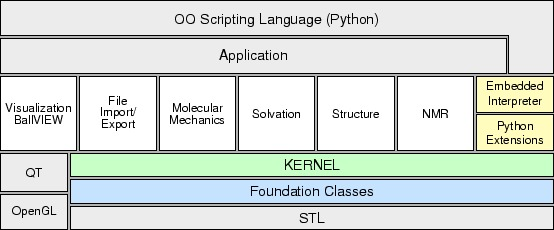
\includegraphics[width=0.5\textwidth]{gfx/BALL-architecture.jpeg}}
	\caption{\ball's architecture is structured in several layers. Upon the standard libary layer are the foundation classes and ontop of them the \texttt{KERNEL}. Several module extend the interface for visualization, file import and expoert, molecular mechanics, solvation, structure and NMR. The C++ written frameworkis extended by Python interface for fast scripting purposes. The figure was taken from the official \ball\ documentation \cite{BALLTutorial}.}
	\label{fig:ball_architecture}
\end{figure}


The main intention for the development of \ball\ as well as for \biochem\ is to generate a framework for rapid prototyping of molecular applications. This section summarizes the key concepts of \ball\ that motivated the design of our project \footnote{An in-depth description of the entire \ball\ framework is beyond the scope of this article. Confer the main publications~\cite{kohlbacher_ballrapid_2000, hildebrandt_ball_2010}  for more details.}\\
The initial work on the \ball\ project started in 1996, resulting in the C++-written library \ball\ and its accompanying molecular viewer, \textit{\ballview}. One reason for \ball's success lies in its sophisticated design; it employs an object-oriented approach with four design goals: \textit{ease of use}, \textit{robustness}, \textit{openness}, and \textit{functionality }
The object-oriented approach facilitates ease of use in combination with the well-documented and intuitive interfaces. As can be seen in Figure~\ref{fig:ball_architecture}, \ball's architecture is structured in several layers:
\begin{itemize}
	
	\item The standard template library (STL) forms its base.
	\item The foundation classes provide general data structures such as hash sets and mathematical objects (e.g., matrices, vectors,...). 
	\item The core consists of the \texttt{KERNEL} classes that contain data structures representing molecular entities.
	
	\item  The basic components represent fundamental functionalities placed atop of this core layer; exceptions include the visualization module that is based on Qt and Open GL \cite{Qt5,OpenGLWebsite}.
	\item Finally, the application layers can be used to develop custom applications or leverage existing tools. \\
\end{itemize}
Hildebrandt \textit{et al.} published an updated version in 2010, featuring  Python bindings alongside installation with the use of CMake as build system -- enhancements that improved usability and openness while allowing easier integration with external packages across different compilers/ operating systems \cite{hildebrandt_ball_2010}. \\

\ball's uniqueness stems from its rich functionality integrated in a single easily extensible open-source platform. Figure \ref{fig:ball_structure} illustrates how \texttt{KERNEL} classes form three frameworks: the general molecular framework, the protein framework, the nucleic acid framework -- all implemented through composite patterns \cite{gamma1994design}. More precisely, the composite class is the base class for all derived classes representing molecular entities such as \texttt{Atom}, \texttt{Protein}, etc. or container classes \texttt{System}, \texttt{AtomContainer}, and so on. \\ 

These frameworks form the basis for the functionalities of the basic components ranging from preprocessing tools (file import/export) to complex analyses (e.g., energy minimization/mapping) alongside advanced solvation methods. 
\ball\ is a well-tested library ensuring robustness of the provided functionalities. \\

\ball's robustness and well-designed structure has contributed significantly to its popularity -- \ball\ used to have one of the biggest user communities in this field.


\begin{figure}[t]
	\centerline{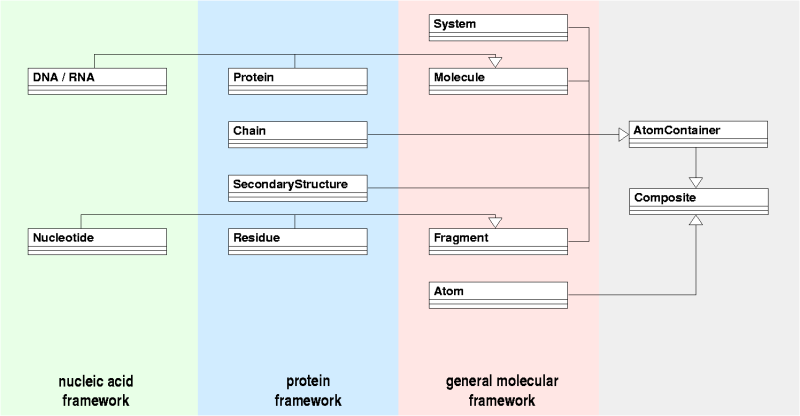
\includegraphics[width=0.5\textwidth]{gfx/KERNEL.png}}
	\caption{UML class diagram of the \texttt{KERNEL} classes. The \texttt{KERNEL} classes form three frameworks and are implemented using the composite pattern\cite{gamma1994design}. The figure was taken from the official \ball\ documentation \cite{BALLTutorial}.}
	\label{fig:ball_structure}
\end{figure}

